\documentclass[11pt,a4paper,twocolumn]{article}
\usepackage[document]{ragged2e}
\usepackage[utf8]{inputenc}
\usepackage{amsmath}
\usepackage{amsfonts}
\usepackage{amssymb}
\usepackage{graphicx}
\usepackage{xcolor}
\usepackage{subfig}
\usepackage[output-decimal-marker={.}]{siunitx}
\usepackage{wrapfig}
\usepackage{lipsum}
\title{\vspace{-2.0cm}Montecarlo Toy for Annihilaiton Discrimination and Hyperfine Measurement}
\author{Adriano Del Vincio, PhD student}
\begin{document}

\twocolumn[
\begin{@twocolumnfalse}  
\maketitle
\begin{abstract}
\centering
A fit procedure to discriminate $\overline{H}$ annihilation on walls from residual gas annihilation has been implemented and tested. Moreover, a Monte Carlo simulation concerning the hyperfine splitting measurement was designed, with the intention of studying the statistical uncertainty and bias of various algorithms to find the onset of the transition $c \rightarrow b$ and $d \rightarrow a$.
\end{abstract}
\end{@twocolumnfalse}
%\hspace{10pt}
]



\section*{Annihilations Discrimination}

The ALPHA magnetic trap is designed to store the anti-hydrogen atoms that are produced during a mixing phase. The mixing phase consists on combining the anti-protons coming from ELENA with the positrons. 
The experiments in ALPHA hinge upon the detection of anti-hydrogen annihilation, to perform measurement pertaining to the asymmetries between matter and antimatter.\\
We take as a reference the hyperfine splitting of anti-hydrogen: the experiment consist on measuring the number of anti-hydrogen released from the magnetic trap subsequent to exposure to laser (microwave light) illumination with different frequencies. Most of the annihilations which are detected occur on the magnetic trap walls. Nevertheless, a certain percentage of this annihilation might arise from annihilation with residual gas. This second contribution is a potential source of background noise for the experiment. In light of this, we have devised a model to characterize and separate the two contribution.
\subsection*{Radius of the Annihilation Vertex}

Data about anti-hydrogen annihilation encompass several variables that are measured by the detectors. In order to distinguish the annihilation on the walls and that originating from residual gas, we have computed the radius (with respect to the center of the trap) $r$ of each annihilation vertex from the $X$ and $Y$ coordinates.
The radius distribution should to differ depending on the type of annihilation: for annihilation on the wall, the radius distribution should manifest a peak corresponding to the radius of the trap, while the events due to residual gas should mostly occur at smaller radius, near the geometric center of the trap.
To model the two contributions, we had different datasets available: 
\begin{itemize}
\item An almost pure annihilation on the walls dataset, taken during the $\SI{2}{\second}$ mixing phase of anti-protons and positions, to which we will refer as \textit{mixing} events.
\item An almost pure annihilation due to residual gas dataset, acquired during the exposure to laser illumination, but far away from the absorption peak (which we will indicate as \textit{UWlosses}).
\item An almost pure dataset of cosmic background events (supposed to be mainly muons) that are reconstructed erroneously as anti-hydrogen vertices. These data are taken when the magnetic trap does not contains the anti-hydrogen atoms.
\end{itemize}

The dataset are analysed separately, to build up different models for the radius distribution for each contribution.

\subsection*{Annihilation on the walls}

The events contained in the \textit{mixing} dataset are supposed to be distributed around the radius of the magnetic trap, with a $\sigma$ given by different contribution, as for example the detector resolution in measuring the vertex coordinates. We have analysed only the events that pass the \textbf{cut 1} selection. The data are fitted assuming a gaussian model, see figure \ref{fig:MixingFit}:

\begin{figure}[hbtp]
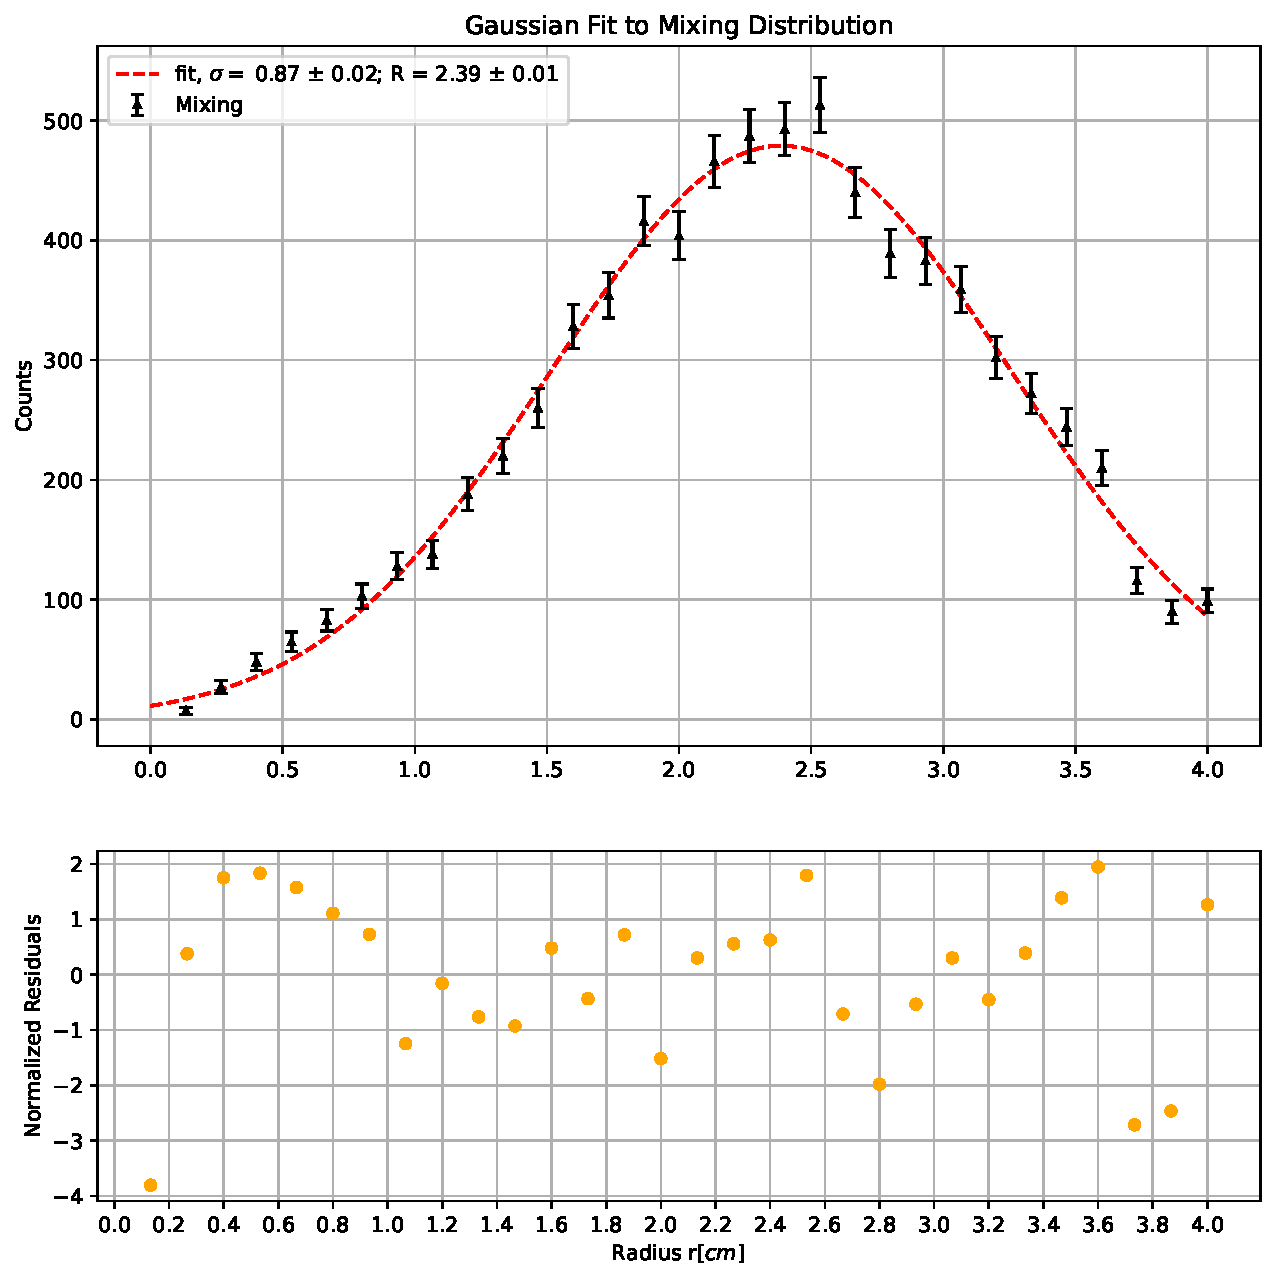
\includegraphics[width = 0.45\textwidth]{../PlotMLEfit/SingleModel/GaussianFitMixing.pdf}
\caption{Radius distribution of the annihilation vertices for the \textit{mixing} dataset. The red line is the gaussian model. On the bottom of the figure the residuals, assuming poissonian fluctuation ($\sigma = \sqrt{Counts}$).}
\label{fig:MixingFit}
\end{figure}

\subsection*{Annihilation due to Residual Gas}

For the Annihilation due to residual gas, we have used a different model compared to the gaussian distribution used before. We have assumed that the anti-hydrogen in the magnetic trap is roughly stored at the center, and that the $X$ and $Y$ coordinates of the annihilation vertices are normal distributed. At this point we assumed also that the $\sigma_{x}$ and $\sigma_{y}$ are equale, so that there is no asymmetry if we consider the two direction $x,y$.


\end{document}